\renewcommand{\theequation}{\theenumi}
\begin{enumerate}[label=\arabic*.,ref=\thesubsection.\theenumi]
\numberwithin{equation}{enumi}
\item We have a triangle as given bellow .First of all we will find out the midpoint of the $\vec AB$ because each median devide the side in two equal part.
 Finding out the point $\vec S $ as given in fig (1.1)...
$\vec S$ is the midpoint of the $\vec P$ and $\vec Q$
\begin{align}
	\vec S &= \frac{\vec P + \vec Q}{2}
\end{align}

Direction vector in the direction of RS

\begin{align}
	\vec {RS}&= \vec{S}  - \vec {R}
\end{align}

  equation of the line going through points $\vec{S}$ and $\vec {R}$ can be given as 
\begin{align}
	\vec {x} &= \vec {R} + \lambda \left(\vec{S}- \vec{R}\right)
	\\
	\vec {x} &= \myvec{4\\5} + \lambda \left(\myvec{0\\2} - \myvec{4\\5}\right)
	\\
	\vec {x} &= \myvec{4\\5} + \lambda \left(\myvec{-4\\-3}\right)
\end{align}
\begin{figure}[!ht]
	\centering
	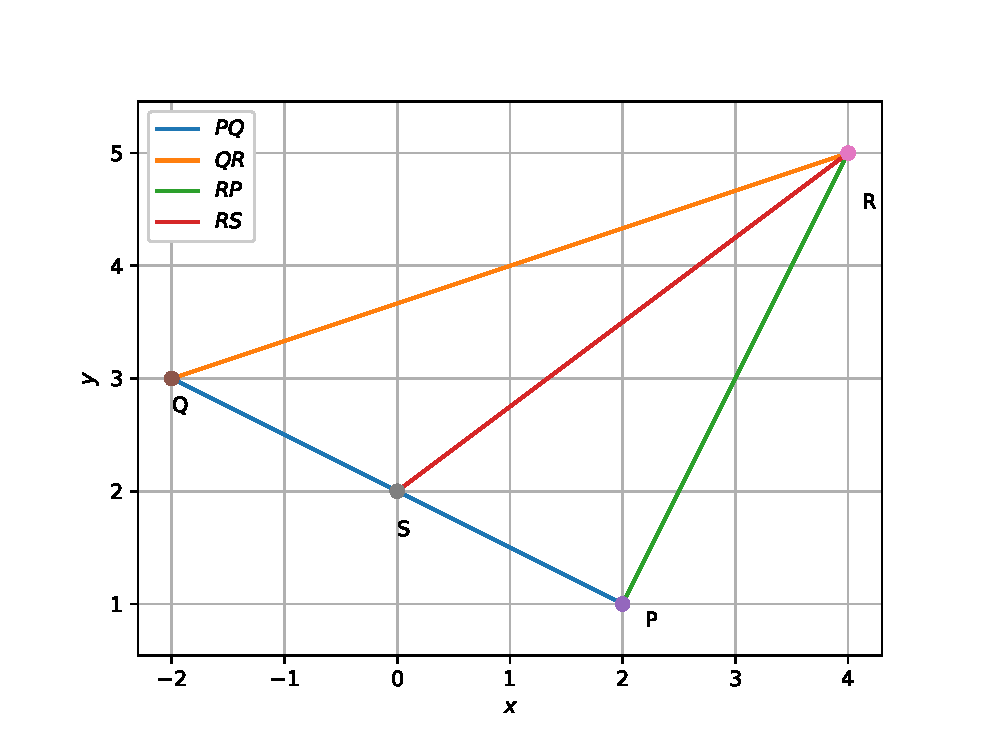
\includegraphics[width=\columnwidth]{./figures/triangle/triangle.eps}
	\caption{triange}
	\label{fig:angle_py}
	Path to pythone code for the above figure
	\begin{lstlisting}
	codes/triangle/triangle.py
	\end{lstlisting}
\end{figure}
\end{enumerate}